\documentclass[11pt]{article}

\usepackage[tt=false, type1=true]{libertine}
\usepackage[varqu]{zi4}
\usepackage[libertine]{newtxmath}
\usepackage[T1]{fontenc}

\usepackage[pdftex]{graphicx}
\usepackage{url}
%\usepackage{mathptmx}		% for times fonts
\usepackage{color,xcolor,colortbl}
\usepackage{algorithm,algorithmic}
\usepackage[mathscr]{euscript}		% DO NOT remove this line, otherwise some symbols may get overload!
\usepackage[letterpaper]{geometry}
\geometry{verbose,tmargin=1in,bmargin=1in,lmargin=1in,rmargin=1in}

\usepackage{mdwmath}
\usepackage{mdwtab}
\usepackage[font=footnotesize]{subfig}

\definecolor{darkblue}{rgb}{0.0,0.0,0.5}
\usepackage[unicode=true,bookmarks=true,bookmarksnumbered=false,bookmarksopen=true,hidelinks=true,colorlinks=true,citecolor=darkblue,linkcolor=black]{hyperref}
	
\usepackage{epstopdf}
\let\openbox\relax
\usepackage{amsthm}
\usepackage{relsize}

\newcommand{\etal}{\textit{et~al.}}
\newcommand{\eg}{\textit{e.g.}}
\newcommand{\ie}{\textit{i.e.}}
\newcommand{\alg}[1]{\mbox{\textsf{#1}}}
\newcommand{\view}[1]{\textsf{{\small VIEW}}_{#1}}

\setlength{\parskip}{0.25em}
\let \labelindent \relax
\usepackage{enumitem}
\setlist[description]{listparindent=\parindent,leftmargin=0em,itemsep=0.75em}
\setlist[itemize]{listparindent=\parindent,itemsep=0em}

\theoremstyle{mytheoremstyle}
\newtheorem{theorem}{Theorem}
\newtheorem{lemma}{Lemma}
\newtheorem{corollary}{Corollary}
\newtheorem{definition}{Definition}
\floatname{algorithm}{Protocol}

\begin{document}

\title{Notes on Consensus Protocols}

\author{Mahdi Zamani\\ Visa Research, Palo Alto, CA \\ \textit{mzamani@visa.com}}
\date{}

\maketitle

\paragraph{Consensus.}
A set of $n$ distributed nodes want to agree on a single value proposed by one of them. In the context of blockchains, consensus often means agreement on a sequence of values similar to an atomic broadcast~\cite{DBLP:journals/corr/CachinV17}. A consensus protocol generally provides the following properties:

\begin{itemize}
	\item \textit{Agreement:} All honest nodes agree on the \emph{same} message.
	\item \textit{Validity:} All honest nodes decide on the the input of some honest node.
	\item \textit{Integrity:} Every honest node decides on at most one value which is the input of some node.
	\item \textit{Termination:} All honest nodes decide on some value.
\end{itemize}

\paragraph{Byzantine Faults.} A node that can deviate arbitrarily from the protocol. Byzantine nodes can vote for both a statement and its contradiction, i.e., make different statements to different nodes to put non-faulty nodes into inconsistent states. When consensus is performed in such a setting, it is often called Byzantine consensus/agreement.

\paragraph{Byzantine Agreement (BA).} One of the participants, called the \emph{leader} or \emph{source}, has an initial value. A Byzantine agreement protocol satisfies the following properties:
\begin{itemize}
	\item \emph{Agreement}: All non-faulty processes must agree on the same value. 
	\item \emph{Validity}: If the source is non-faulty, then the agreed upon value by all the non-faulty nodes must be the same as the initial value of the leader.
	\item \emph{Termination}: Each non-faulty process must eventually decide on a value.
\end{itemize}

\paragraph{Interactive Consistency (IC)~\cite{pease80reaching}.} Each participant has an initial value. All non-faulty participants must agree on a vector of values, one for each participant. More formally:
\begin{itemize}
\item \emph{Agreement}: All honest parties must agree on the same array of values $A[v_1,...,v_n]$. 
\item \emph{Validity}: If party $i$ is honest and its input is $v_i$, then all honest parties agree on $v_i$ for $A[i]$. If party $i$ is faulty, then honest parties can agree on any value for $A[i]$.
\item \emph{Termination}: Each honest party must eventually decide on $A$.
\end{itemize}

\paragraph{Equivalence of Consensus Variants.} If any of the consensus variants (Byzantine agreement, consensus, and interactive consistency) has a solution, then all of them have a solution. For example, IC can be achieved from BA by run BA $n$ times, one with each participant as the leader. Also, consensus can be achieved from IC by running IC, then outputting the first element of the vector.

\paragraph{Safety and Liveness Guarantees.} \emph{Safety} means that all non-faulty nodes agree on the same outcome. \emph{Liveness} means that the non-faulty nodes will make progress during the course of the protocol. Safety can be trivially achieved by making no forward progress at all from an initial state. Liveness can be trivially achieved by making progress unsafely by just letting each node decide on arbitrary outcomes. Neither of these guarantees are useful by themselves.

\paragraph{Consensus Termination.} A consensus protocol terminates when all non-faulty participants have terminated. If all non-faulty participants terminate in the same round, then we call they have achieved an \emph{immediate agreement}. Otherwise, we call they have achieved an \emph{eventual agreement}~\cite{fischer}.
Pease~\etal~\cite{pease80reaching} show that at most ${t<n/2}$ nodes can be faulty for the Byzantine agreement to be solvable. Also, they show that if messages are not authenticated using a digital signature scheme, then at most ${t<n/3}$ nodes can be faulty.

\paragraph{CAP Theorem.} It is impossible for a distributed data store to simultaneously provide more than two out of the following three properties: 
\begin{itemize}
	\item \textbf{Consistency:} Every read receives the most recent write or an error.
	\item \textbf{Availability:} Every request receives a (non-error) response.
	\item \textbf{Partition Tolerance:} The system works even if an arbitrary number of messages being dropped (or delayed).
\end{itemize}
In other words, in the presence of a network partition, the system can only guarantee either consistency or availability. Existing decentralized systems (such as cryptocurrencies) work by compromising between availability and consistency.

\paragraph{Authenticated Byzantine Agreement.}
When messages exchanged between the participants are signed using a digital signature scheme, the protocol is called authenticated Byzantine agreement. This assumption requires that the author of a signed message be determined by anyone holding the message, regardless of where it came from (this is often called the \emph{non-repudiation} property). Therefore, message authentication codes (MACs) cannot be solely used to provide authenticated BA. Such an assumption makes synchronous Byzantine agreement solvable when $f<n/2$~\cite{srini2017}. The intuition behind this is that corrupted nodes can no longer simulate the actions of honest nodes because the use of digital signatures prevents impersonations.

Dolev and Strong~\cite{Dolev:Strong:83} show that authenticated BA can be achieved in $t+1$ rounds and $O(nt)$ messages using the following algorithm:

\begin{enumerate}
	\item In each round, each node signs the value and sends it to only the participants who have not signed it yet.
	\item After $t$ rounds, each message has $t$ signatures on it. Hence, each correct value has been seen by all the correct participants after $t+1$ rounds.
\end{enumerate}

\paragraph{Message and Round Impossibilities of BA.}
For deterministic protocols, it is shown that $t+1$ rounds are needed for both unauthenticated and authenticated BA~\cite{FischerLynch81,Dolev:1982:STOC}. Also, any (deterministic) authenticated BA requires exchanging $\Omega(nt)$ messages~\cite{dolev:reischuk:82}.

\paragraph{FLP Impossibility~\cite{FLP}.} Deterministic consensus in the asynchronous setting is impossible even with one crash failure. This is because it is impossible to distinguish a failed process from a very slow one, so processes remain ambivalent when deciding. To avoid this impossibility and/or to achieve practicality, the protocol may be allowed to provide probabilistic safety or liveness guarantees. In the latter case, the protocol is said to provide \emph{eventual liveness} (or \emph{eventual consistency}) since nodes can decide on a value with probability one but with no time bound.

\paragraph{Bracha-Toueg Impossibility~\cite{Bracha:Toueg:1983}.} There is no (probabilistic) asynchronous consensus protocol resilient to $t \geq n/3$ malicious nodes. See Figure~\ref{fig:bounds}.

\begin{figure}
	\centering
	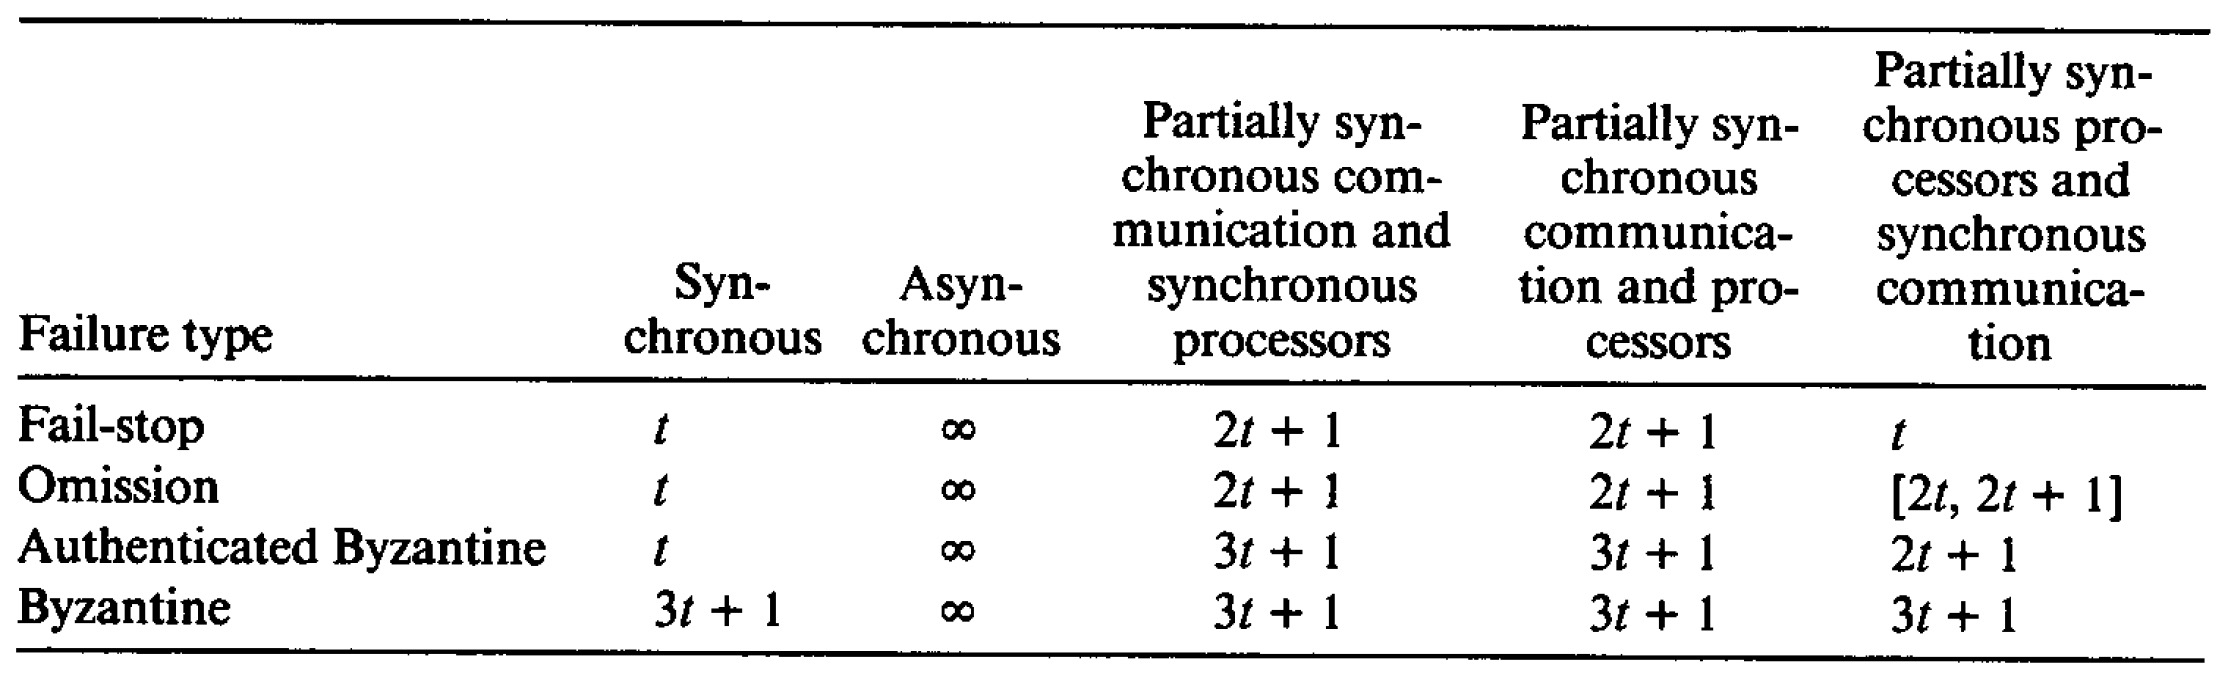
\includegraphics[width=0.9\linewidth]{bounds}
	\caption{Smallest number of nodes for which $t$-resilient consensus protocol exists~\cite{dwork:1988:cpp}.}
	\label{fig:bounds}
\end{figure}

\paragraph{Broadcast Channel.} If a broadcast channel is available, then the Byzantine agreement problem is trivial: each player simply broadcasts their value and then honest players decide on the majority value.

\paragraph{Atomic Broadcast.}
A set of distributed nodes agree on a sequence of values~\cite{AtomicBroadcast:1993}. Consensus and atomic broadcast are equivalent because a sequence of consensus instances provides atomic broadcast. An atomic broadcast protocol generally provides the following properties:
\begin{itemize}
	\item \textit{Agreement:} All honest nodes eventually receive the \emph{same} message.
	\item \textit{Validity:} If an honest node broadcasts a message, then all honest nodes eventually receive it.
	\item \textit{Integrity:} All honest nodes receive the same message exactly once.
	\item \textit{Total Order:} An honest node receives $m_1$ before $m_2$ if and only if the sender sends $m_1$ before $m_2$.
\end{itemize}

\paragraph{Reliable Broadcast.}

\paragraph{State-Machine Replication.}
A protocol that runs among a set of nodes to agree on a sequence of requests based on a deterministic state machine that implements the logic of a service to be replicated among the nodes.

\paragraph{Eventual Synchrony.} Introduced by Dwork~\cite{dwork:1988:cpp}, it models an asynchronous network that may delay messages among honest nodes arbitrarily, but eventually behaves synchronously delivering all messages within a \emph{fixed} but \emph{unknown} time bound. It is widely accepted as a realistic model for designing robust distributed systems~\cite{DBLP:journals/corr/CachinV17}.

\paragraph{Partial Synchrony.} Similar to eventual synchrony but with probabilistic network behavior over time~\cite{dwork:1988:cpp}.

\paragraph{View-Change Protocols.} Some consensus protocols such as Paxos~\cite{lamport:1998:Paxos}, Raft~\cite{raft:2014}, and PBFT~\cite{pbft:99} proceed in \emph{epochs} (a.k.a., \emph{views}), where a \emph{leader} (a.k.a., the \emph{primary}) is responsible for the progress of the protocol. When a node (a.k.a., a \emph{replicate} or \emph{backup}) suspects that the leader is faulty, the node broadcasts a \textsc{View-Change} message to replace the leader. The new leader has to gather at least $2f+1$ signed \textsc{View-Change} messages, to broadcast a \textsc{New-View} message. A Byzantine leader cannot violate safety (\ie, cause inconsistencies) but can violate liveness (\ie, prevent progress) by not proposing. In PBFT~\cite{pbft:99}, every honest participant monitors the current leader, and if a new message is not proposed after some time, the honest participant requests a new leader.

\paragraph{Byzantine Generals Problem.} A commanding general orders its lieutenant generals to attack or to surrender. Some of the generals are traitors. The goal is:
\begin{itemize}
	\item All loyal lieutenants obey the same order, or
	\item If the commanding general is loyal, then every loyal lieutenant obeys the order he sends.
\end{itemize}

Why is consensus among generals important? Because, halfhearted attack by a few generals would be worse than a coordinated attack or a coordinated retreat. Pease et al.~\cite{pease80reaching} prove $3f+1$ parties are necessary to achieve agreement in this problem.

\bibliographystyle{alpha}
\bibliography{../../secbib/secbib}			% pull from https://github.com/mahdiz/secbib

\end{document}